% !TEX TS-program = lualatex
% !TEX encoding = UTF-8 Unicode

\documentclass[12pt, letterpaper]{article}

%%BIBLIOGRAPHY- This uses biber/biblatex to generate bibliographies according to the 
%%Unified Style Sheet for Linguistics
\usepackage[main=american, german]{babel}% Recommended
\usepackage{csquotes}% Recommended
\usepackage[backend=biber,
             style=unified,
             maxcitenames=3,
             maxbibnames=99,
             natbib,
             url=false]{biblatex}
\addbibresource{Library.bib}
\setcounter{biburlnumpenalty}{100}  % allow URL breaks at numbers
%\setcounter{biburlucpenalty}{100}   % allow URL breaks at uppercase letters
%\setcounter{biburllcpenalty}{100}   % allow URL breaks at lowercase letters

%%TYPOLOGY
\usepackage[svgnames]{xcolor} % Specify colors by their 'svgnames', for a full list of all colors available see here: http://www.latextemplates.com/svgnames-colors
%\usepackage[compact]{titlesec}
%\titleformat{\section}[runin]{\normalfont\bfseries}{\thesection.}{.5em}{}[.]
%\titleformat{\subsection}[runin]{\normalfont\scshape}{\thesubsection}{.5em}{}[.]
\usepackage[hmargin=1in,vmargin=1in]{geometry}  %Margins
\usepackage{graphicx} % 
\usepackage{stackengine} %Package to allow text above or below other text, Also helpful for HG weights 
\usepackage{fontspec} %Selection of fonts must be ran in XeLaTeX
\usepackage{amssymb} %Math symbols
\usepackage{amsmath} % Mathematical enhancements for LaTeX
\usepackage{setspace} %Linespacing
\usepackage{multicol} %Multicolumn text
\usepackage{enumitem} %Allows for continuous numbering of lists over examples, etc.
\usepackage{multirow} %Useful for combining cells in tablesbrew 
\usepackage{booktabs}
\usepackage{hanging}
\usepackage{fancyhdr} %Allows for the 
\pagestyle{fancy}
\fancyhead[L]{\textit{QP Defense Handout}} 
\fancyhead[R]{\textit{\today}} 
\fancyfoot[L,R]{} 
\fancyfoot[C]{\thepage} 
\renewcommand{\headrulewidth}{0.4pt}
\setlength{\headheight}{14.5pt} % ...at least 14.49998pt
% \usepackage{fourier} % This allows for the use of certain wingdings like bombs, frowns, etc.
% \usepackage{fourier-orns} %More useful symbols like bombs and jolly-roger, mostly for OT
\usepackage[colorlinks,allcolors={black},urlcolor={blue}]{hyperref} %allows for hyperlinks and pdf bookmarks
% \usepackage{url} %allows for urls
% \def\UrlBreaks{\do\/\do-} %allows for urls to be broken up
\usepackage[normalem]{ulem} %strike out text. Handy for syntax
\usepackage{tcolorbox}
\usepackage{datetime2}
\usepackage{caption}
\usepackage{subcaption}

%%FONTS
\setmainfont{Libertinus Serif}
\setsansfont{Libertinus Sans}
\setmonofont[Scale=MatchLowercase]{Libertinus Mono}

%%PACKAGES FOR LINGUISTICS
%\usepackage{OTtablx} %Generating tableaux with using TIPA
\usepackage[noipa]{OTtablx} % Use this one generating tableaux without using TIPA
%\usepackage[notipa]{ot-tableau} % Another tableau drawing packing use for posters.
% \usepackage{linguex} % Linguistic examples
% \usepackage{langsci-linguex} % Linguistic examples
\usepackage{langsci-gb4e} % Language Science Press' modification of gb4e
% \usepackage{langsci-avm} % Language Science Press' AVM package
\usepackage{tikz} % Drawing Hasse diagrams
% \usepackage{pst-asr} % Drawing autosegmental features
\usepackage{pstricks} % required for pst-asr, OTtablx, pst-jtree.
% \usepackage{pst-jtree} %Syntax tree draawing software
% \usepackage{tikz-qtree} % Another syntax tree drawing software. Uses bracket notation.
\usepackage[linguistics]{forest} % Another syntax tree drawing software. Uses bracket notation.
% \usepackage{ling-macros} % Various linguistic macros. Does not work with linguex.
% \usepackage{covington} % Another linguistic examples package.
\usepackage{leipzig} % Offers support for Leipzig Glossing Rules

%%LEIPZIG GLOSSING FOR ZAPOTEC
\newleipzig{el}{el}{elder} % Elder pronouns
\newleipzig{hu}{hu}{human} % Human pronouns
\newleipzig{an}{an}{animate} % Animate pronouns
\newleipzig{in}{in}{inanimate} % Inanimate pronouns
\newleipzig{pot}{pot}{potential} % Potential Aspect
\newleipzig{cont}{cont}{continuative} % Continuative Aspect
% \newleipzig{pot}{pot}{potential} % Potential Aspect
\newleipzig{stat}{stat}{stative} % Potential Aspect
\newleipzig{and}{and}{andative} % Andative Aspect
\newleipzig{ven}{ven}{venative} % Venative Aspect
% \newleipzig{res}{res}{restitutive} % Restitutive Aspect
\newleipzig{rep}{rep}{repetitive} % Repetitive Aspect

%%TITLE INFORMATION
\title{TITLE}
\author{Mykel Loren Brinkerhoff}
\date{\today}

%%MACROS
\newcommand{\sub}[1]{\textsubscript{#1}}
\newcommand{\supr}[1]{\textsuperscript{#1}}
\providecommand{\lsptoprule}{\midrule\toprule}
\providecommand{\lspbottomrule}{\bottomrule\midrule}
\newcommand{\fittable}[1]{\resizebox{\textwidth}{!}{#1}}

\makeatletter
\renewcommand{\paragraph}{%
  \@startsection{paragraph}{4}%
  {\z@}{0ex \@plus 1ex \@minus .2ex}{-1em}%
  {\normalfont\normalsize\bfseries}%
}
\makeatother
\parindent=10pt


\begin{document}

%%If using linguex, need the following commands to get correct LSA style spacing
%% these have to be after  \begin{document}
    % \setlength{\Extopsep}{6pt}
    % \setlength{\Exlabelsep}{9pt}%effect of 0.4in indent from left text edge
%%

%% Line spacing setting. Comment out the line spacing you do not need. Comment out all if you want single spacing.
%\doublespacing
%\onehalfspacing

\begin{center}
    {\Large \textbf{Laryngeal Complexity in Santiago Laxopa Zapotec}}
	% \footnote{I am grateful to Fe Silva-Robles and  Raúl Díaz Robles for sharing their time and language expertise. I am also grateful to Grant McGuire,  Jaye Padgett, Rachel Walker, Maziar Toosarvandani, Ben Eischens, Kim Tan, and Zach Horton for their help and discussions during all stages of this project. This project branched off of a collaboration with Jack Duff and Maya Wax Cavallaro. Various parts of this project were previously shared in joint presentations with Jack Duff and Maya Wax Cavallaro.
	
	% This work was supported in part by the National Science Foundation under Grant No. 2019804, the Humanities Institute at UC Santa Cruz, and the Jacobs Research Funds.}
    \vspace{6pt}

    Mykel Loren Brinkerhoff
\end{center}
%\maketitle
%\maketitleinst
\thispagestyle{fancy}

% \tableofcontents

%------------------------------------
\section{Introduction} \label{sec:Introduction}
%------------------------------------

\begin{itemize}
    \item Most work on tonal languages has been based on descriptions of Southeast and Far East Asian languages.
	\item This has lead to strong claims being made about what is possible for languages that contain tone and phonation \citep{masicaDefiningLinguisticArea1976,thurgoodVietnameseTonogenesisRevising2002,yipTone2002,enfieldArealLinguisticsMainland2005,michaudComplexTonesEast2012,brunelleTonePhonationSoutheast2016}. 
	\item The main claim from many of these authors is that tone and phonation are codependent.
	\item An example for this type of co-occurrence between tone and phonation is Mandarin's Tone 3 which is frequently associated with creaky voice \citep{hockettPeipingPhonology1947,}. 
	\item This claim has also been made in the reverse.
	 \begin{itemize}
		\item Breathy voice stereotypically appears with high pitch and creaky voice stereotypically appears with low pitch \citep{eslingVoiceQualityLaryngeal2019}.
	\end{itemize}
	\item Research into Mesoamerican languages, however, shows that these claims are too strong or exaggerated \citep{suarezMesoamericanIndianLanguages1983,campbellMesoAmericaLinguisticArea1986,silvermanLaryngealComplexityOtomanguean1997,dicanioPhoneticsPhonologySan2008,espositoVariationContrastivePhonation2010, campbellOtomangueanHistoricalLinguistics2017a,campbellOtomangueanHistoricalLinguistics2017}. 
	\item Most languages of the Oto-Manguean language family exhibits independent tone and phonation \citep{silvermanLaryngealComplexityOtomanguean1997,blankenshipTimeCourseBreathiness1997,blankenshipTimingNonmodalPhonation2002,ariza-garciaPhonationTypesTones2018}. 
	\item This has lead some researchers to propose that tone and phonation is phased/ordered with respect to each other in what is termed the Laryngeal Complexity Hypothesis \citep{silvermanLaryngealComplexityOtomanguean1997,blankenshipTimeCourseBreathiness1997,blankenshipTimingNonmodalPhonation2002}. 
	\item A summary of this proposal is discussed in Section~\ref{sec:Silverman}.
	\item Using Santiago Laxopa Zapotec, an Otomanguean language spoken in Santiago Laxopa, Ixtlán, Oaxaca, Mexico, I show that:
	\begin{itemize}
		\item There are clear ordering effects between the different phonation types.
		\begin{itemize}
			\item Laryngealized vowels have a modal phonation in the middle of the vowel
			\item Checked and breathy vowels have non-modal phonation at the end of the vowel. 
		\end{itemize} 
		\item Using a Generalized Additive Mixed Model \citep{hastieGeneralizedAdditiveModels1986,woodGeneralizedAdditiveModels2017}, I show that the Laryngeal Complexity Hypothesis correctly characterizes the interaction between tone and phonation in Santiago Laxopa Zapotec. 
	\end{itemize}
\end{itemize}

%------------------------------------
\section{Laryngeal Complexity Hypothesis} \label{sec:Silverman}
%------------------------------------

\begin{itemize}
	\item The Laryngeal Complexity Hypothesis (LCH) has its origin in work from \citet{silvermanLaryngealComplexityOtomanguean1997,blankenshipTimeCourseBreathiness1997,blankenshipTimingNonmodalPhonation2002}.
	\item The LCH claims that languages that have both tone and phonation need them to be phased/ordered with respect to each other. 
	\item This is required because it is assumed that the same mechanism for tone is also responsible for phonation. 
	\begin{itemize}
		\item Tone is the rate of vocal fold vibration. 
		\item \citet{ladefogedPreliminariesLinguisticPhonetics1971,gordonPhonationTypesCrosslinguistic2001} argued that phonation exists on a single dimension ranging from opened vocal folds to closed vocal folds. 
	\end{itemize} 
	\item The variation in how open or closed the vocal folds are correspond to whether or not the sound produced is breathy or creaky. 
	\item \citet{ladefogedPreliminariesLinguisticPhonetics1971,gordonPhonationTypesCrosslinguistic2001} summarized this assumption in the diagram found in Figure~\ref{fig:Phonation}.
\end{itemize}
\begin{figure}[!h]
	\centering
	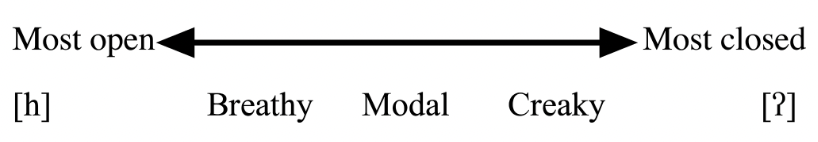
\includegraphics[width=.6\textwidth]{../Phonation.png}
	\caption{Simplified one-deminsional model for phonation. Based on \citet{ladefogedPreliminariesLinguisticPhonetics1971,gordonPhonationTypesCrosslinguistic2001}}.
	\label{fig:Phonation}
\end{figure}
\vspace{-2ex}
\begin{itemize}
	\item Because the same organ is responsible for these two different phenomena there is a mismatch in trying to produce both at the same time. 
	\item The LCH assumes that there needs to be a strict ordering in the glottal gestures. 
	\item If the gestures were overlapped there will be a perturbation of the tone and the listeners will not be able to reliably differentiate what the tone is.
	\item The LCH assumes that there is a close link between production and perception. 
	\item This assumption places the responsibility on making sure the acoustic cues are the most perceptually salient on the speaker. 
	\item In Figure~\ref{fig:GlottalGestures}, which is taken from \citet{dicanioCoarticulationToneGlottal2012}, the cue for tone is represented by the Pitch Target and the Glottal Gesture represents the gestures needed to produce phonation. 
\end{itemize}
	\begin{figure}[!ht]
		\centering
		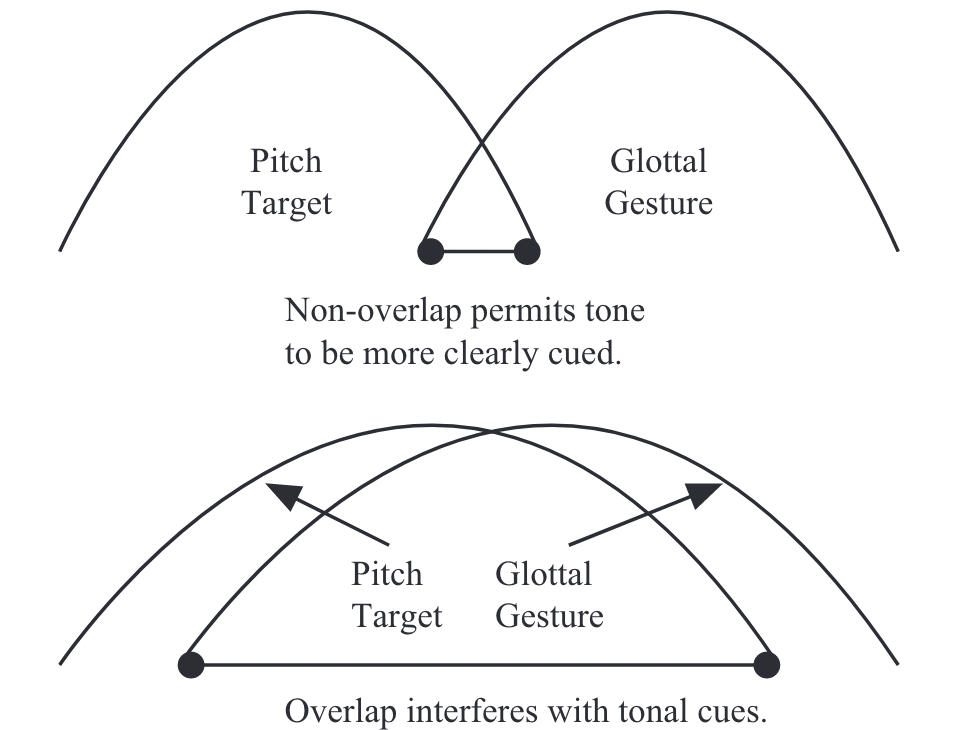
\includegraphics[width=.5\textwidth]{../Gestures.png}
		\caption{Representation taken from \citet{dicanioCoarticulationToneGlottal2012}.}
		\label{fig:GlottalGestures}
	\end{figure}
\begin{itemize}
	\item \citet{dicanioCoarticulationToneGlottal2012} found that when the magnitude of coarticulation for glottal consonants occurs on the vowels there is a strong correlation between the magnitude of overlap and the amount of perturbation in the f0 signal. If, however, the degree of overlap was minor then the acoustic signal had little to no perturbation.
	\item Jalapa Mazatec is a language with both contrastive tone and phonation and \citet{garellekAcousticConsequencesPhonation2011} validated the claims made by the LCH, in that tone and phonation seemed to be ordered with each other when it comes to at least one of the phonation types.
\end{itemize}

%------------------------------------
\section{Santiago Laxopa Zapotec} \label{sec:SLZ}
%------------------------------------

\begin{itemize}
    \item Santiago Laxopa Zapotec (SLZ), endonym \textit{Dille'xhunh Laxup}, is a a Northern Zapotec language spoken by approximately 1000 people in the municipality of Santiago Laxopa, Ixtlán, Oaxaca, Mexico and in diaspora communities in Mexico and the United States \citep{adlerAcousticsPhonationTypes2016,adlerDerivationVerbInitiality2018,foleyForbiddenCliticClusters2018,foleyExtendingPersonCaseConstraint2020}.
    \item Closely related to San Bartolomé Zoogocho Zapotec \citep{longDiccionarioZapotecoSan2005,sonnenscheinDescriptiveGrammarSan2005} and shares a high level of mutual intelligibility with it.
    \item SLZ is similar to other Zapotecan languages in distinguishing lenis and fortis consonants \citep[e.g.,][]{nellisFortisLenisCajonos1980,jaegerFortisLenisQuestion1983,uchiharaFortisLenisGlides2016}.
\end{itemize}

\begin{table}[!h]
	\centering
	\caption{Consonant inventory for Santiago Laxopa Zapotec}
	\label{tab:SLZcons}
	\fittable{
	\begin{tabular}{llcccccccc}
	\lsptoprule
		  &  & bilabial & alveolar  & post- & retroflex & palatal &velar &labio-  &  uvular \\
		 &&&&alveolar&  &&&velar& \\
	\midrule
	stop 		& lenis   & b  & d  & & & & g & gʷ & \\
				& fortis  & p  & t  & & & & k & kʷ & \\
	fricative   & lenis   &    & z  & ʒ & ʐ &  & &  & ʁ \\
		        & fortis  &    & s  & ʃ & ʂ & ç & & & \\
	affricate 	& lenis   &    & d͡z & & & & & & \\
				& fortis  &    & t͡s & & t͡ʃ & & & & \\
    nasal    	& lenis   &	   & n  & & & & & & \\
				& fortis  &	mː & nː & & & & & & \\
	lateral  	& lenis   &    & l & & & & & & \\
				& fortis  &    & lː & & & & & & \\
	trill		& 		  &    & r & & &  & &  & \\ 			
	approximate & 		  &    & & & & & & w & \\ 
	\lspbottomrule
	\end{tabular}
	}
\end{table}

\begin{itemize}
    \item SLZ has a standard five vowel inventory. 
\end{itemize}

\begin{table}[!h]
	\centering
	\caption{Vowel qualities in Santiago Laxopa Zapotec.}
    \label{tab:SLZvowels}
	\begin{tabular}{lccc}
	\lsptoprule
	&  front& central  & back \\
	\midrule
	high   	&  i  &     &   u \\
	mid    	&  e  &   	& 	o \\
	low   	&     &  a 	&	  \\
	\lspbottomrule
	\end{tabular}
\end{table}

\begin{itemize}
	\item These five vowels, additionally, appear with one of four different phonation types which will be discussed in greater detail in Section~\ref{sec:Phonation}.
\end{itemize}

%------------------------------------
\subsection{Tone in Santiago Laxopa Zapotec} \label{sec:Tone}
%------------------------------------

\begin{itemize}
    \item Similar to other Otomanguean languages, SLZ is tonal \citep{suarezMesoamericanIndianLanguages1983,campbellMesoAmericaLinguisticArea1986,silvermanLaryngealComplexityOtomanguean1997,campbellOtomangueanHistoricalLinguistics2017a,campbellOtomangueanHistoricalLinguistics2017}.
    \item SLZ has five distinct tonal patterns that appear on the syllables of nouns, see Table~\ref{tab:tones}. 
\end{itemize}

\begin{table}[!h]
	\centering
	\caption{Examples of the five tonal patterns observed in the Santiago Laxopa Zapotec words.}
	\label{tab:tones}
	\begin{tabular}{lllll}
	\lsptoprule
	High   	&  a\supr{H}  &  \textit{xha}   &  [ ʐa\supr{H} ] & `clothing.\textsc{poss}'\\
	Mid    	&  a\supr{M}  &  \textit{lhill} 	& [ liʒ\supr{M} ] & `house.\textsc{poss}' \\
	Low   	&  a\supr{L}  &  \textit{yu'} 	&	 [ çuˀ\supr{L} ] & `earth'\\
	Rising	&  a\supr{MH}  &  \textit{yu'u} 	&	[ çuˀu\supr{MH} ] & `quicklime (Sp. cal)' \\
	Falling &  a\supr{HL}  &  \textit{yu'u}  &	[ çuˀu\supr{HL} ] &	`house' \\
	\lspbottomrule
	\end{tabular}
\end{table}

\begin{itemize}
	\item These five tonal patterns are illustrated in Figures~\ref{fig:FSRTonePlot} for one SLZ speakers. 
	\item Figures~\ref{fig:FSRTonePlot} shows the five tonal contrasts averaged for each tonal contrast from the onset to ending of the vowel. 
	\item The first 20-25\% of Figures~\ref{fig:FSRTonePlot} can be ignored due to the influence of consonantal transitions. 
\end{itemize}

\begin{figure}[!ht]
	\centering
	\includegraphics[width=0.9\textwidth]{../FSRTonePlot.png}
	\caption{Tonal contrasts for FSR averaged and time normalized. Each line in this graph represents the average of approximately 10 syllables for each tonal pattern. }
	\label{fig:FSRTonePlot}
\end{figure}

%------------------------------------
\subsection{Phonation in Santiago Laxopa Zapotec} \label{sec:Phonation}
%------------------------------------

\begin{itemize}
	\item Zapotecan languages commonly make use of contrastive phonation on vowels \citep[e.g.,][]{avelinobecerraTopicsYalalagZapotec2004,longDiccionarioZapotecoSan2005,avelinoAcousticElectroglottographicAnalyses2010,lopeznicolasEstudiosFonologiaGramatica2016,chavez-peonInteractionMetricalStructure2010}.
	\item SLZ is no different and has four contrastive phonation types: modal /a/, breathy /a̤/, checked /aˀ/, and laryngealized /aˀa/. 
\end{itemize}

\ea \label{ex:YA} Four-way near minimal phonation contrast
	\ea \textit{yag}  [çag\supr{L}] `tree; wood; almúd (unit of measurement approximately 4kg)'
	\ex \textit{yah}  [ça̤\supr{L}] `metal; rifle; bell'
	\ex \textit{cha'}  [t͡ʃaˀ\supr{L}]  `a cooking pot'
	\ex \textit{ya'a}  [çaˀa\supr{L}]  `market'
	\z 
\z 
\begin{itemize}
	\item Breathy phonation on vowels is characterized by a raspy quality throughout the whole vowel or a portion toward the end of the vowel, see Figure~\ref{fig:BreathyVowel}. 
\end{itemize}

\begin{figure}[!h]
	\centering
	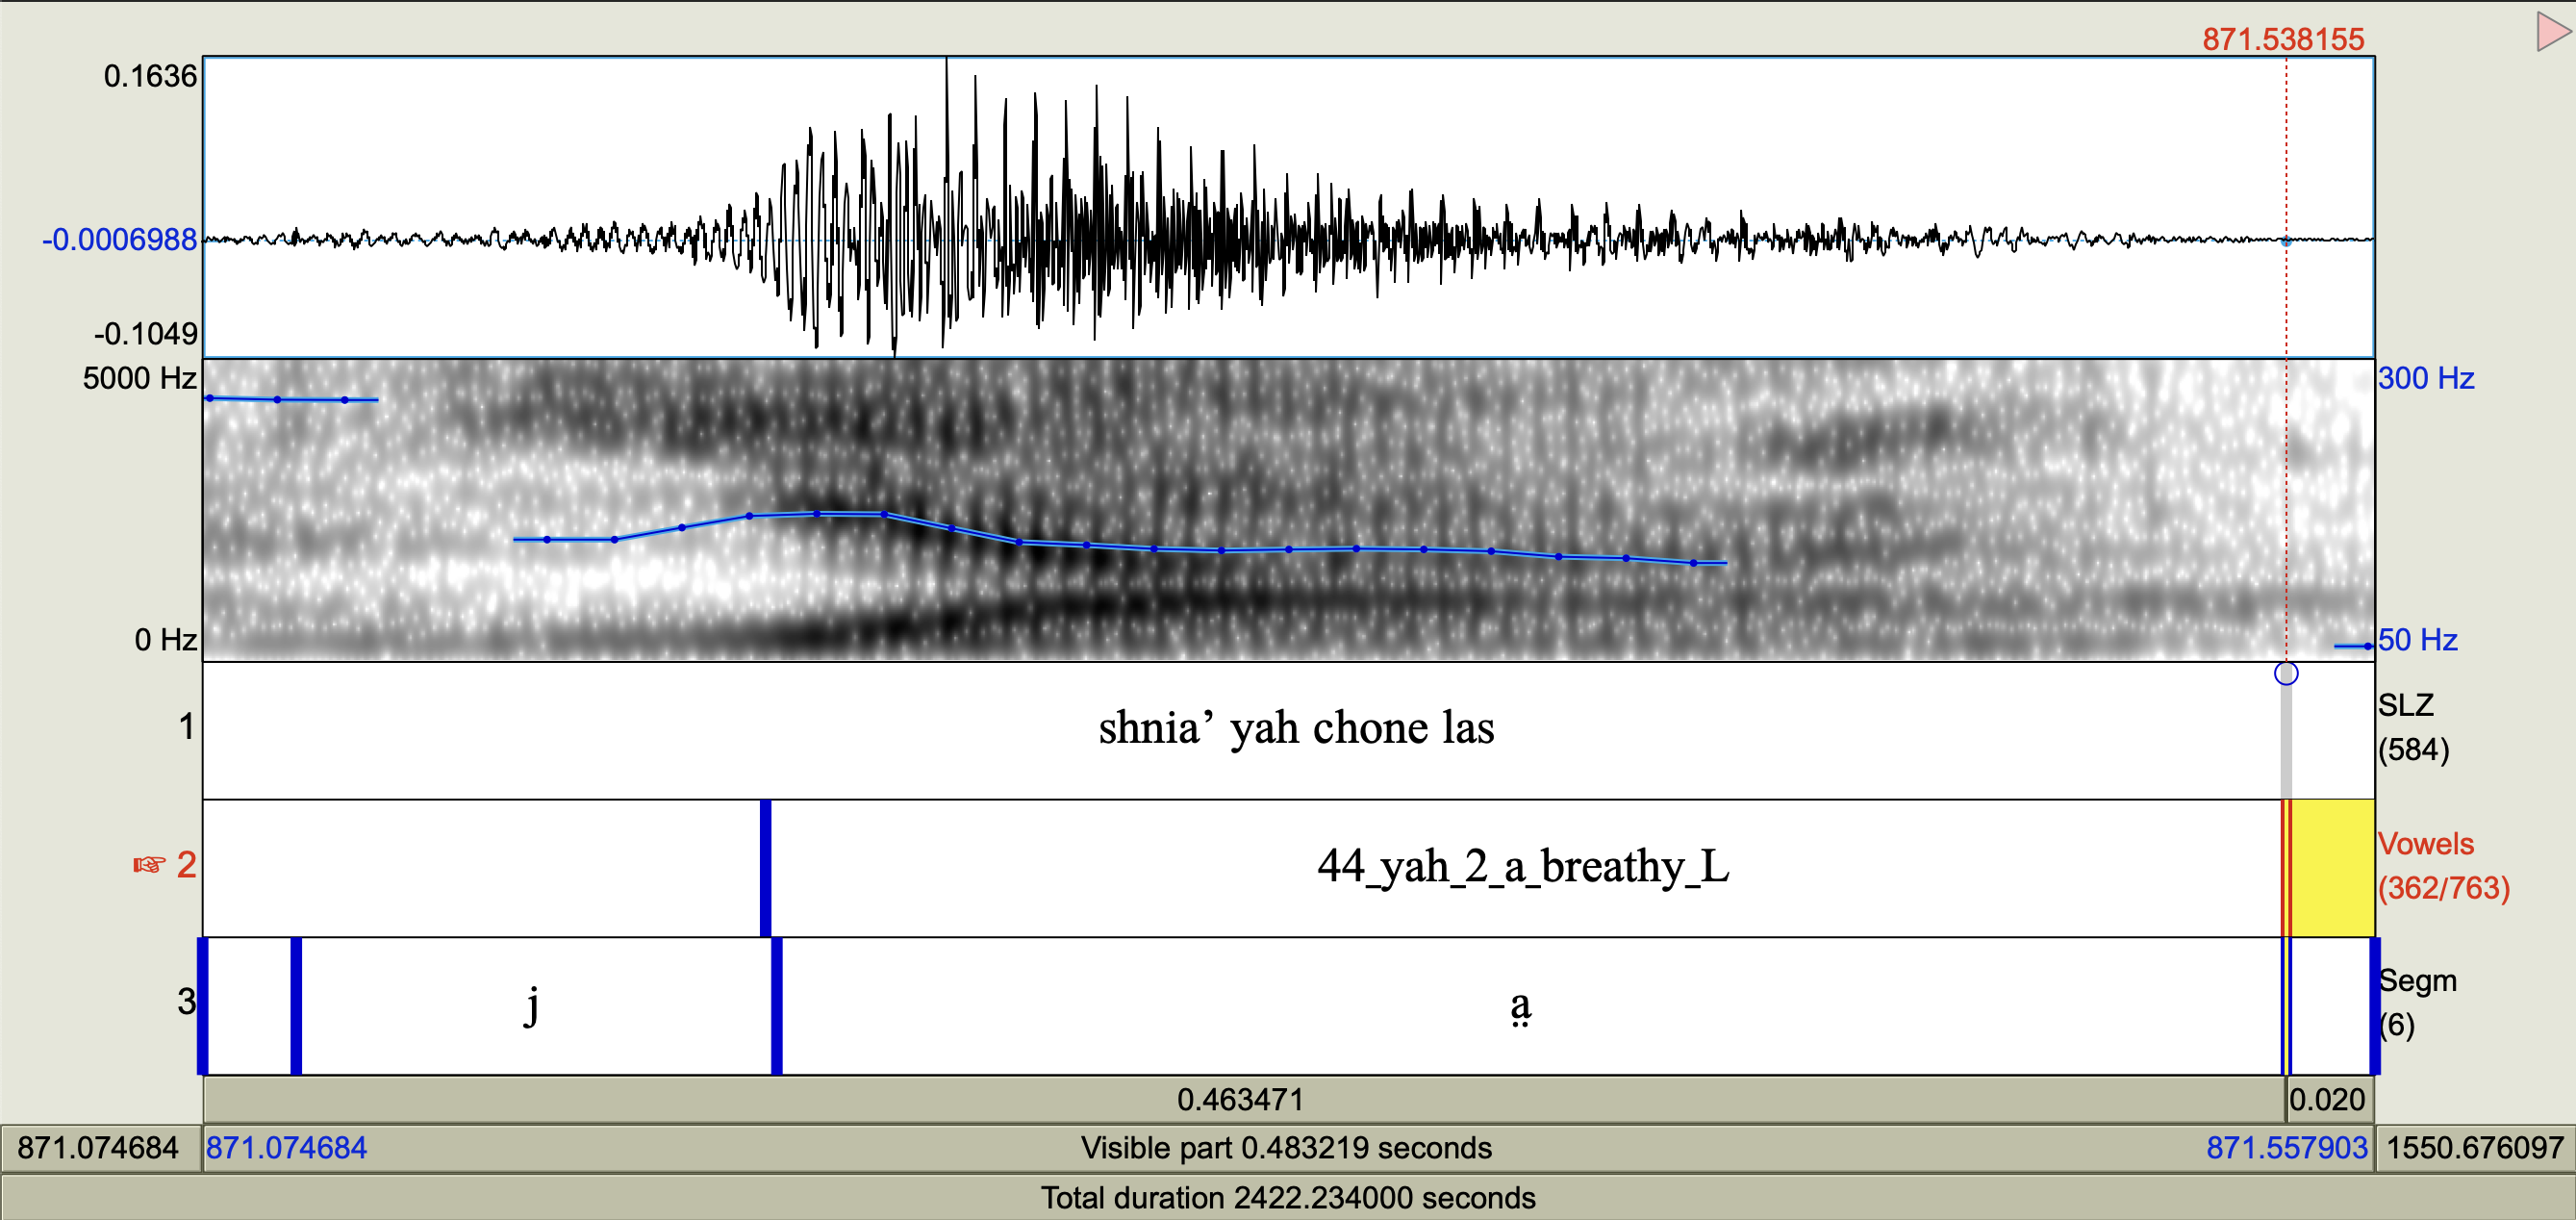
\includegraphics[width=0.9\textwidth]{../yah.png}
	\caption{FSR's breathy vowel in the word \textit{yah} `metal; rifle'}
	\label{fig:BreathyVowel}
\end{figure}

\begin{itemize}
	\item Checked vowels on the other hand are characterized by an abrupt glottal closure which cuts the vowel short. This phonation is sometimes only realized as a very short period of creakiness at the end of the vowel, see Figure~\ref{fig:CheckedVowel}.  
\end{itemize}

\begin{figure}[!h]
	\centering
	% [INSERT YA SPECTROGRAM AND WAVEFORM]
	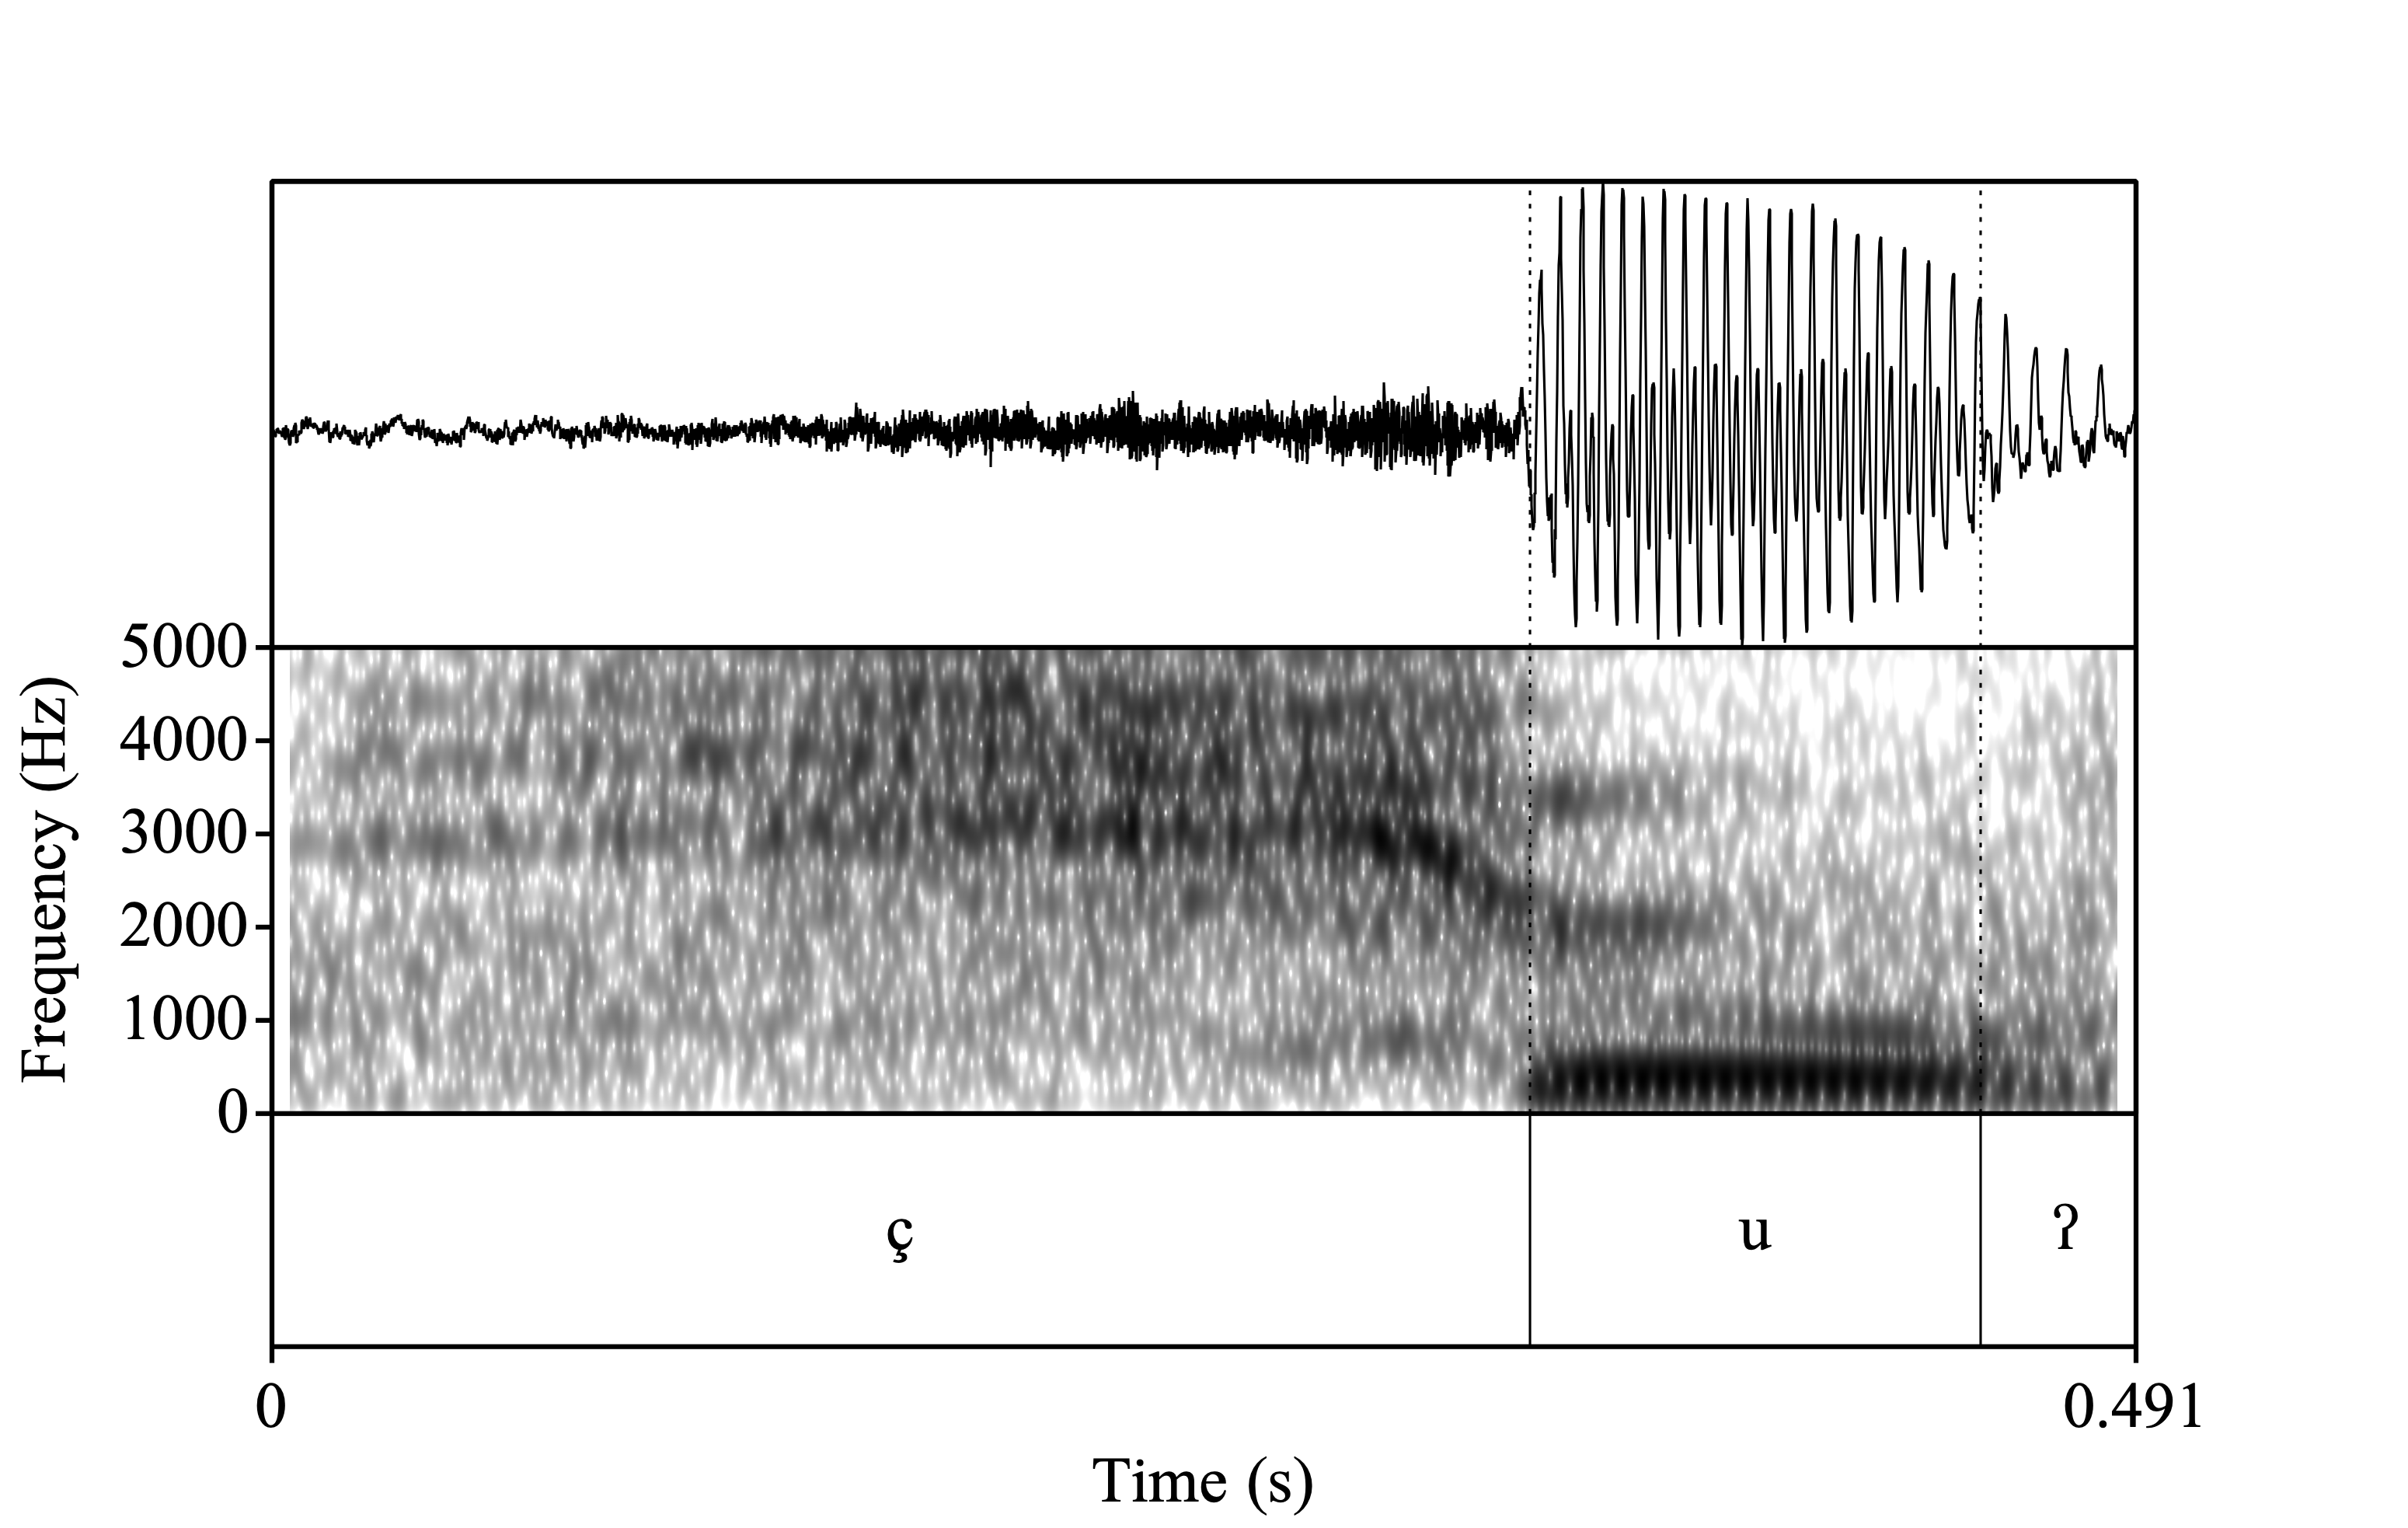
\includegraphics[width=0.9\textwidth]{../RD_yu'.png}
	\caption{RD's checked vowel in the word \textit{yu'} `earth'}
	\label{fig:CheckedVowel}
\end{figure}

\begin{itemize}
	\item Laryngealized vowels are quite common in Zapotecan languages and have received a wide number of different names. 
	\item Previous descriptions have used terms such as broken, rearticulated, interrupted, and creaky \citep{longDiccionarioZapotecoSan2005,avelinobecerraTopicsYalalagZapotec2004,avelinoAcousticElectroglottographicAnalyses2010,sonnenscheinDescriptiveGrammarSan2005,adlerAcousticsPhonationTypes2016,ariza-garciaPhonationTypesTones2018}.  
	\item In addition to a wide number of different names these vowels also exhibit a wide range of allophones.
	\item \citet{avelinoAcousticElectroglottographicAnalyses2010} found in the closely realted Yalálag Zapotec that among his consultants there were at least four different pronunciations as seen in Table~\ref{tab:laryngeal}. 
\end{itemize}

\begin{table}[!h]
	\centering
	\caption{Layngealized Vowels in Yalálag Zapotec}
	\label{tab:laryngeal}
	 \begin{tabular}{ll}
	\lsptoprule
	/VˀV/	&  [VʔV]  \\
			&  [VV̰V]   \\
			&  [VV̰ːV̆]  \\
			&  [VV̰V̰]	\\
	\lspbottomrule
	\end{tabular}
\end{table}

\begin{itemize}
	\item In SLZ, this vowel is also highly variable.
	\item One consultant does rearticulation, where there is a full glottal stop in the middle of the vowel, or creaky voice. 
	\item This alternation seemed to be in free variation but there was a greater tendency to creak in words with a L tone, such as \textit{xa'ag} [ʂa̰ːx] `topil'\footnote{A topil is a type of government office in traditional Oaxacan communities somewhat akin to a sheriff. }, see Figure~\ref{fig:FSRLaryngeal} for a comparison between this consultant's pronunciation of the laryngealized vowels.
\end{itemize}

\begin{figure}[!h]
	\centering
	\begin{subfigure}{.5\textwidth}
		\centering
		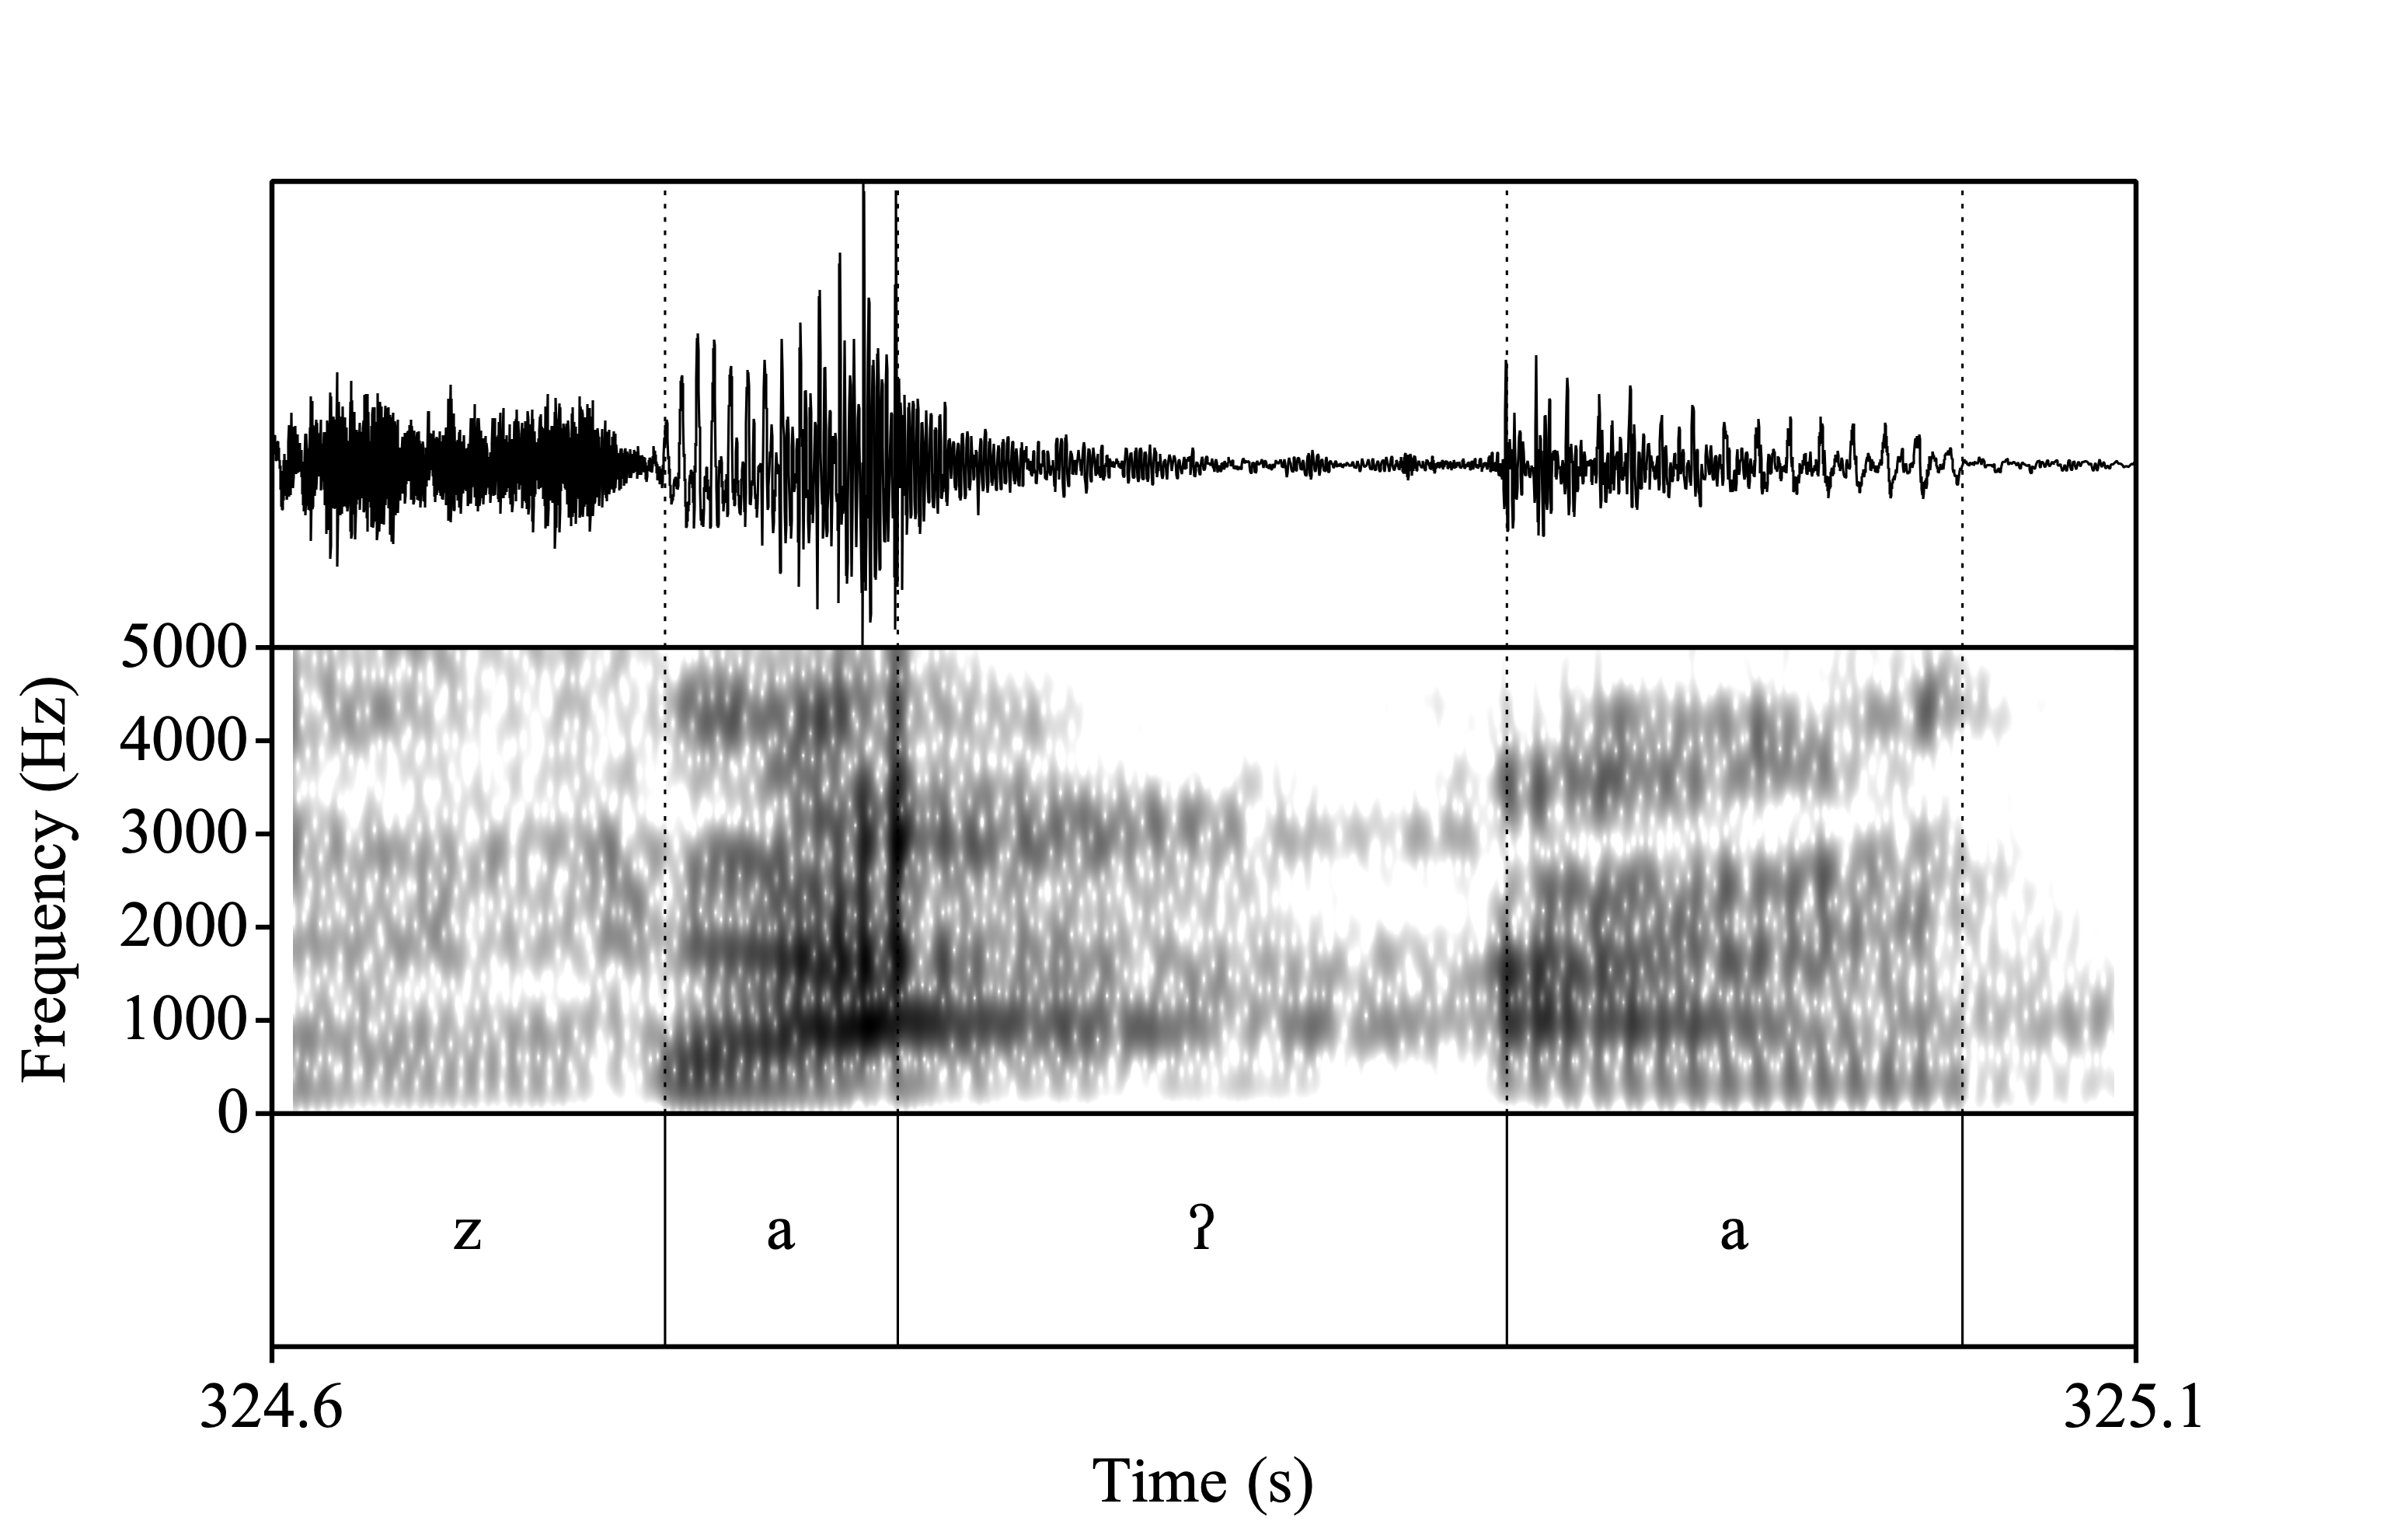
\includegraphics[width=\linewidth]{../za'a.png}
		\caption{\textit{za'a} `corncob'}
		\label{fig:za'a}
	\end{subfigure}%
	\begin{subfigure}{.5\textwidth}
		\centering
		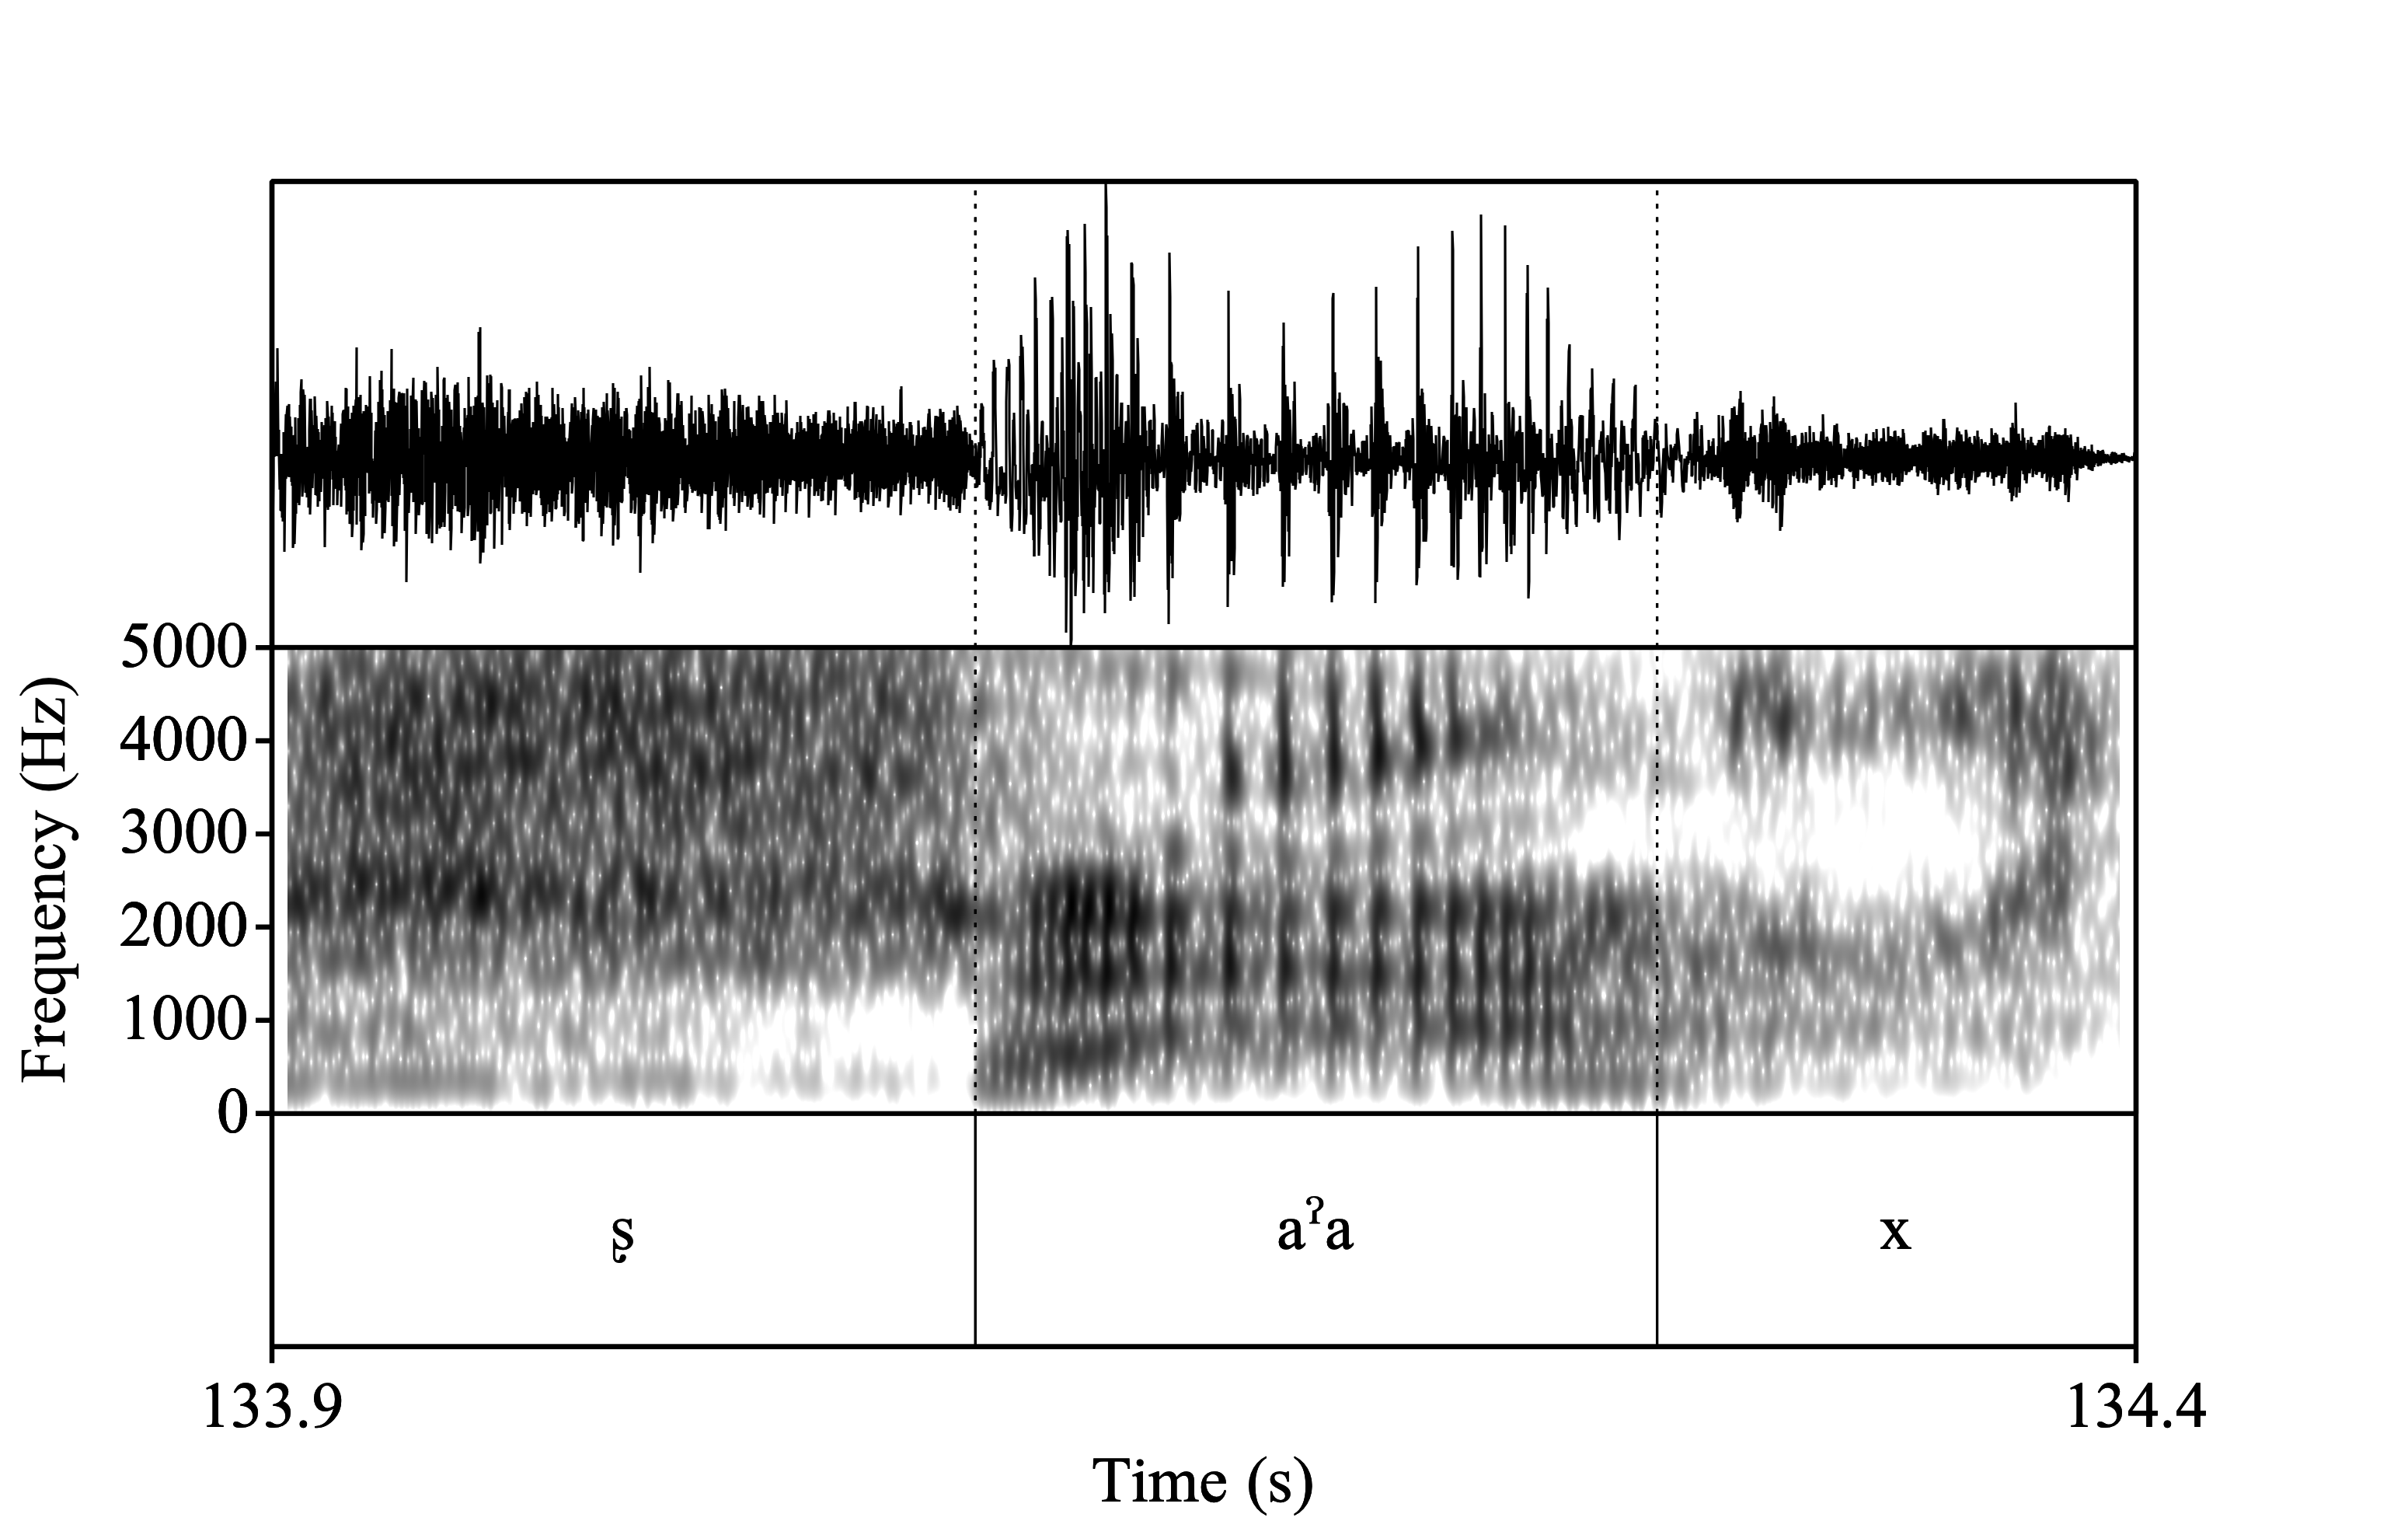
\includegraphics[width=\linewidth]{../xa'ag.png}
		\caption{\textit{xa'ag} `topil'}
		\label{fig:xa'ag}
	\end{subfigure}	
	\caption{Comparison of FSR's laryngealized vowels in \textit{za'a} `corncob' and \textit{xa'ag} `topil'}
	\label{fig:FSRLaryngeal}
\end{figure}

\begin{itemize}
	\item Another consultant only ever produces creaky voice for these vowels regardless of the tone with the word.
\end{itemize}

% \begin{figure}[!h]
% 	\centering
% 	\begin{subfigure}{.5\textwidth}
% 		\centering
% 		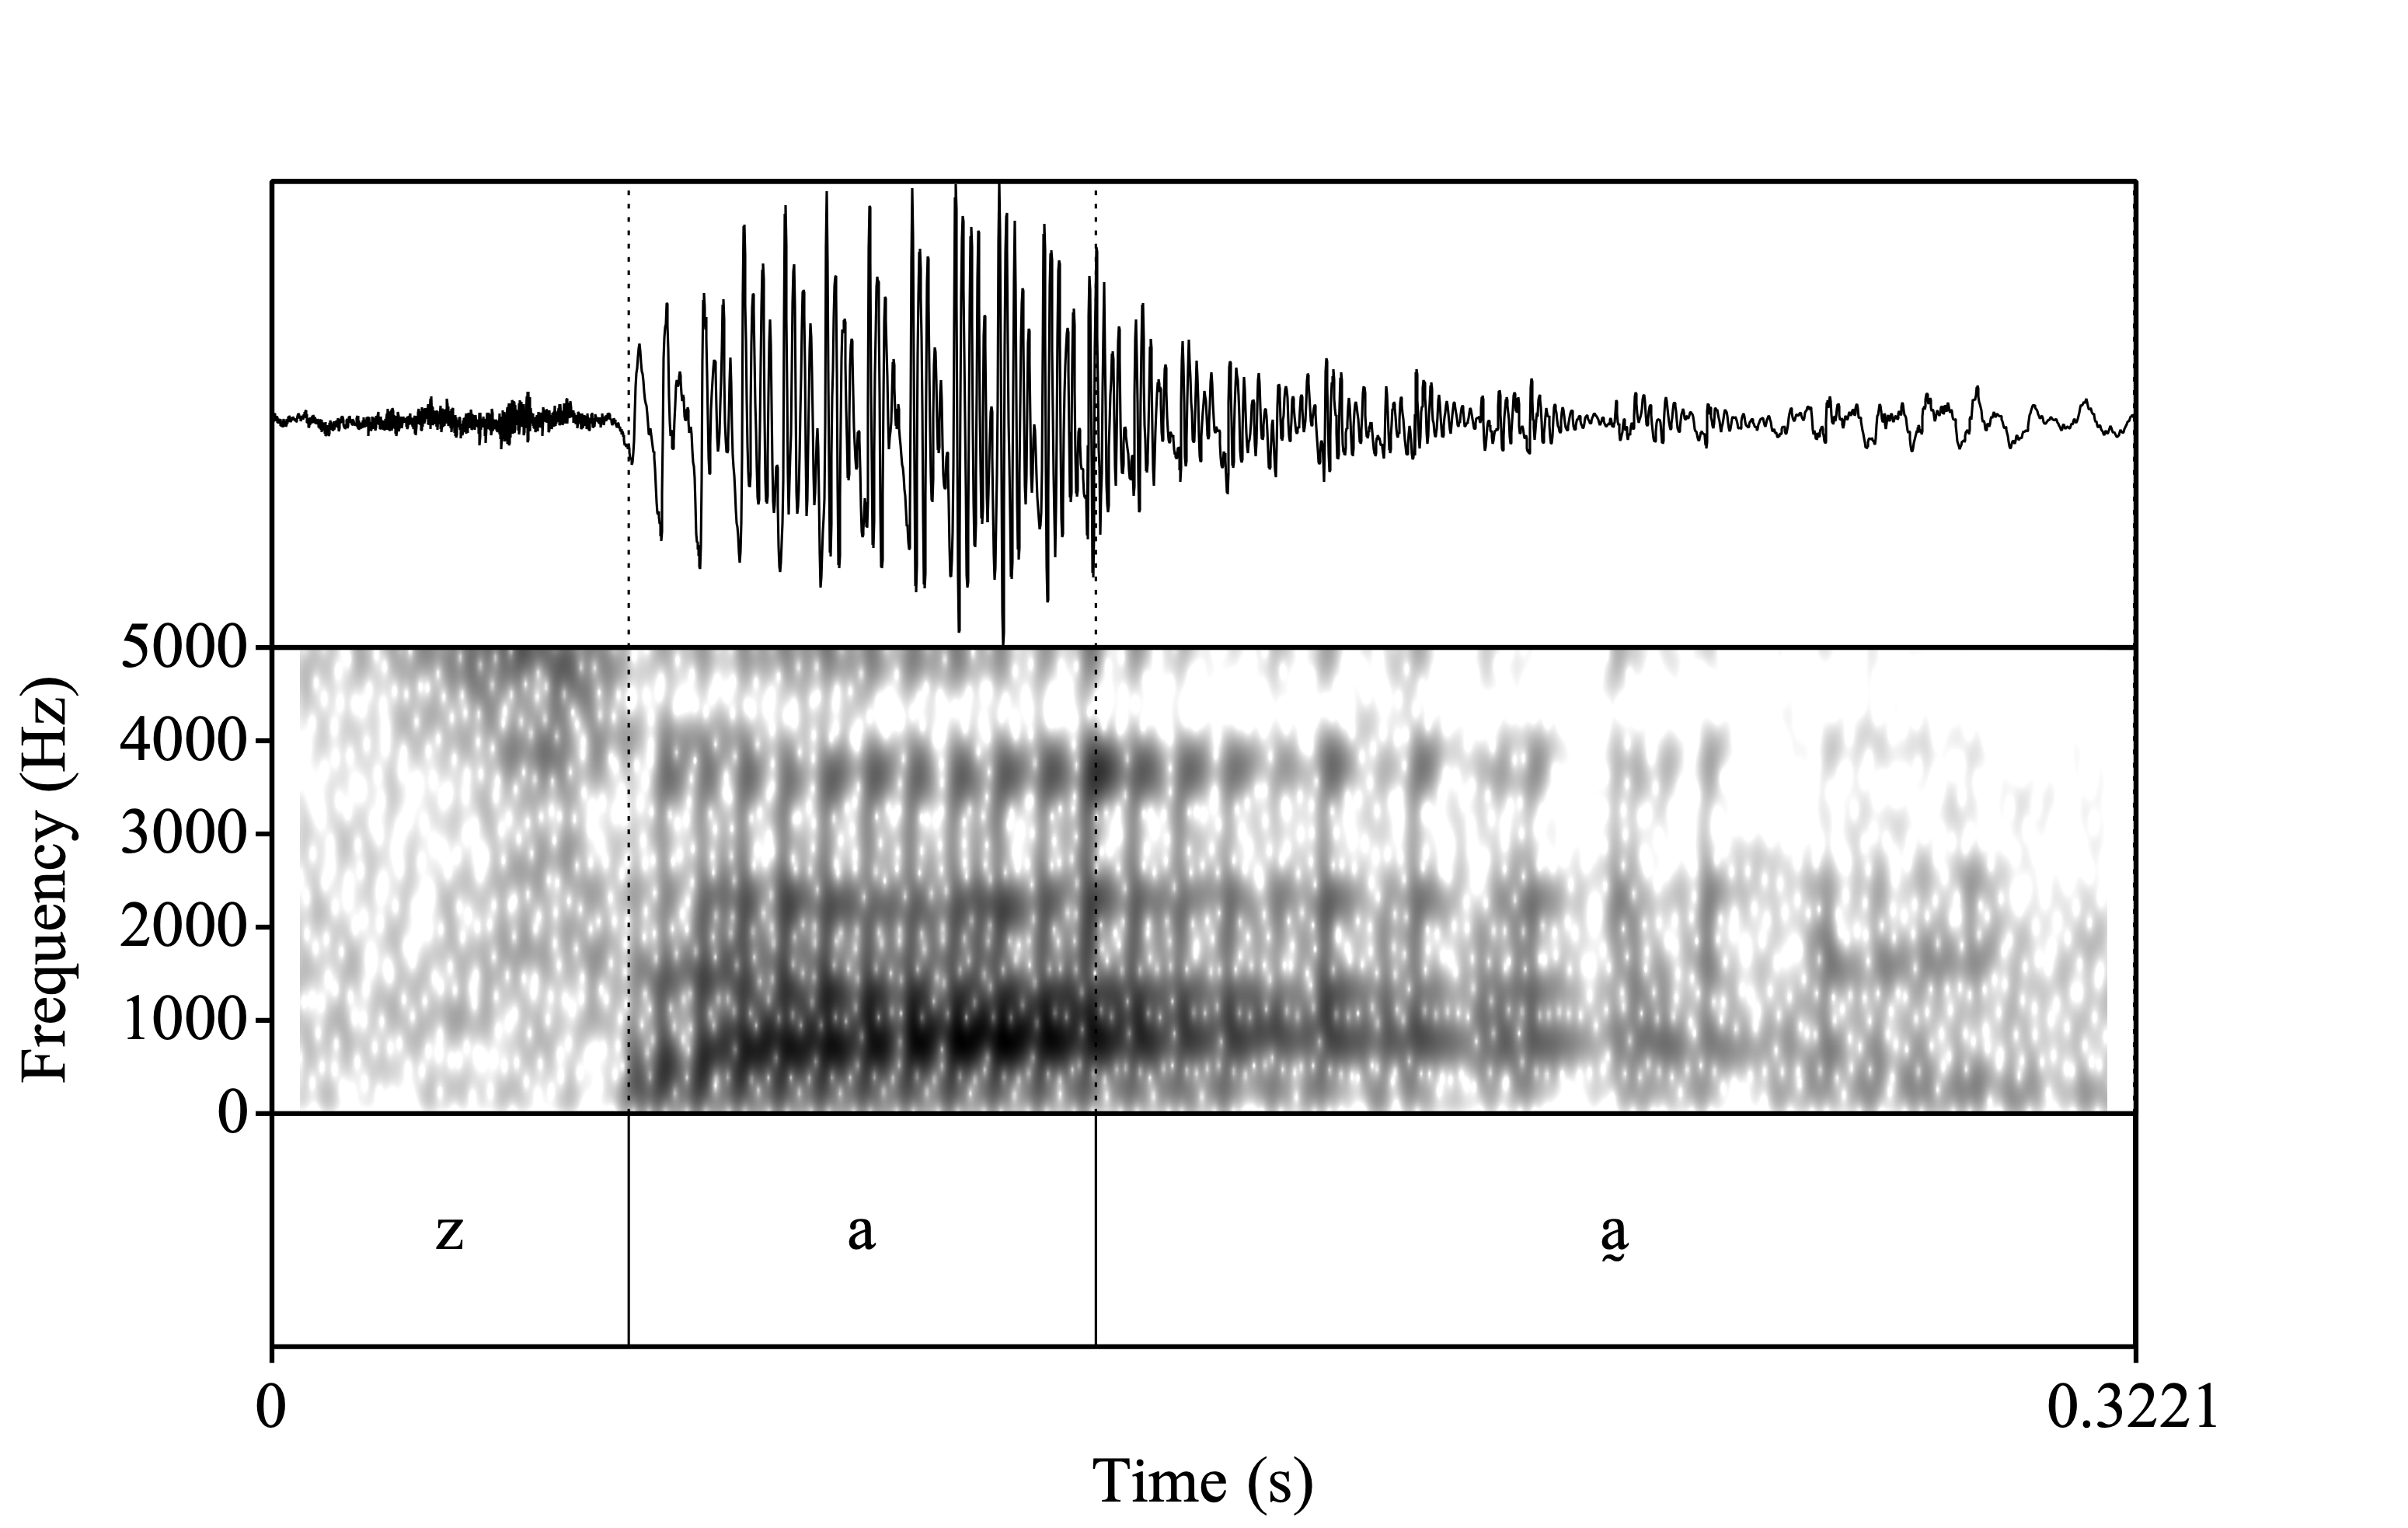
\includegraphics[width=\linewidth]{RD_za'a.png}
% 		\caption{\textit{za'a} `corncob'}
% 		\label{fig:za'a}
% 	\end{subfigure}%
% 	\begin{subfigure}{.5\textwidth}
% 		\centering
% 		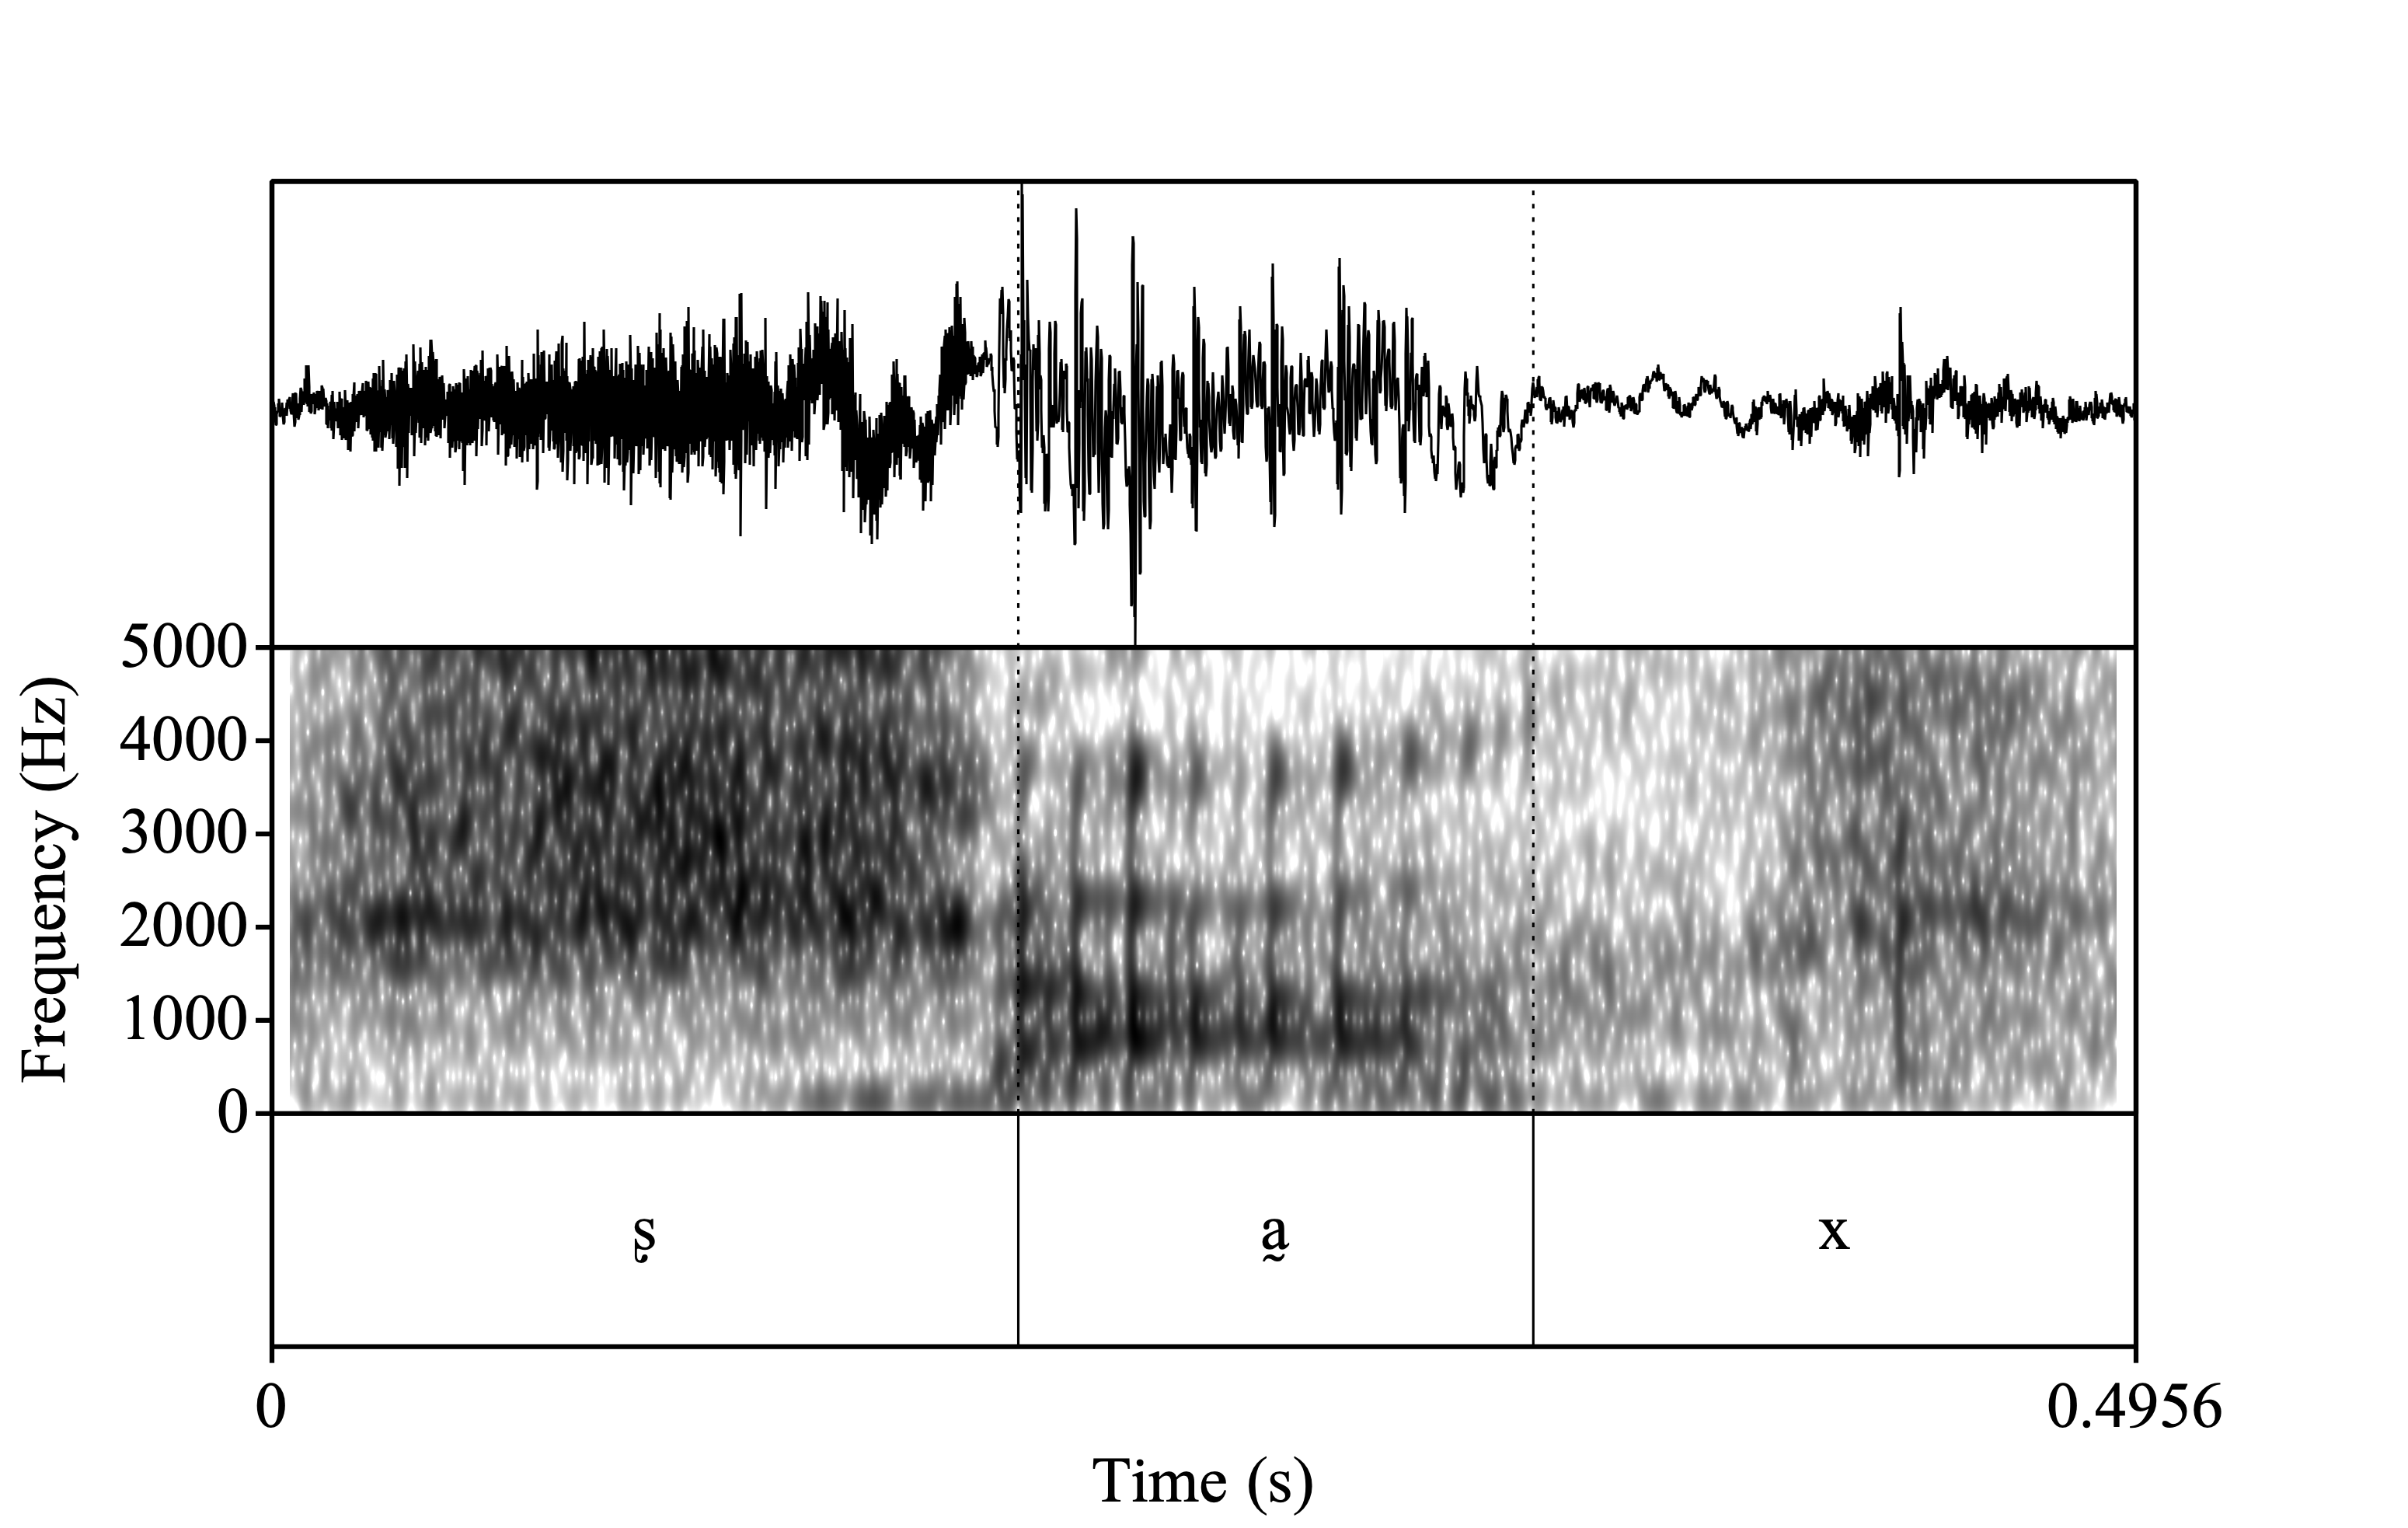
\includegraphics[width=\linewidth]{RD_xa'ag.png}
% 		\caption{\textit{xa'ag} `topil'}
% 		\label{fig:xa'ag}
% 	\end{subfigure}
% 	\caption{Comparison of RD's laryngealized vowels in \textit{za'a} `corncob' and \textit{xa'ag} `topil'}
% 	\label{fig:RDLaryngeal}
% \end{figure}

% \begin{itemize}
% 	\item Further investigations 
% \end{itemize}
%------------------------------------
\subsection{Interaction of tone and phonation in Santiago Laxopa Zapotec} \label{sec:TonePhonation}
%------------------------------------

\begin{table}[!ht]
	\centering
	\caption{SLQZ tone and phonation interactions \citep{chavez-peonInteractionMetricalStructure2010}.}
	\label{tab:SLQZ}
	 \begin{tabular}{lcccc}
	  \lsptoprule
					  &	 \textbf{Modal}  & \textbf{Breathy} & \textbf{Creaky} & \textbf{Interrupted} \\
		  High	& ✔︎ & -- & ✔︎ & ✔︎ \\
		  Low & ✔︎ & ✔︎ & ✔︎ & ✔︎ \\
		  Falling & ✔︎ & ✔︎ & ✔︎ & ✔︎ \\
		  Rising & ✔︎ & -- & -- & -- \\
	  \lspbottomrule
	 \end{tabular}
\end{table}

\begin{table}[!h]
	\caption{Number of unique syllables for each interaction of tone and phonation in the data.}
	\label{tab:ToneVoiceQuality}
	\centering

	\begin{tabular}{lcccc}
	\lsptoprule
		& \textbf{Modal} & \textbf{Breathy} & \textbf{Checked} & \textbf{Laryngealized} \\
	\hline
	High		& ✔︎ & -- & ✔︎ & ✔︎ \\
	Mid			& ✔︎ & ✔︎  & ✔︎ & ✔︎ \\
	Low			& ✔︎ & ✔︎  & ✔︎ & ✔︎ \\
	High-Low	& ✔︎ & ✔︎  & ✔︎ & ✔︎ \\
	Mid-High	& ✔︎ & ✔︎  & --	& ✔︎ \\
	\lspbottomrule
	\end{tabular}
\end{table}


%------------------------------------
\section{Methodology} \label{sec:Methods}
%------------------------------------

\begin{itemize}
	\item 18 native language speakers of SLZ who live in Santiago Laxopa, Ixtlán, Oaxaca, Mexico took part in this study (7 male). 
	\item Because of the COVID-19 pandemic data collection was conducted remotely using Zencastr\footnote{\href{https://zencastr.com/}{https://zencastr.com/}}, a professional podcasting website, (44.1kHz, 16-bit) or in-person outside in a well ventilated location, using a Zoom H4n handheld recorder (44.1kHz, 16-bit).
	\item The speakers were asked to say 80 words that varied for phonation and tone three times in isolation and three times in the carrier phrase shnia' X chone las.
\end{itemize}

%------------------------------------
%BIBLIOGRAPHY
%------------------------------------

%\singlespacing
% \nocite{*}
\printbibliography[heading=bibintoc]

\end{document} 